\documentclass[12pt]{article}
\usepackage{amsmath}
\usepackage{amsfonts}
\usepackage{amssymb}
\usepackage{graphicx}
\usepackage[margin=1in]{geometry}
\usepackage{listings}
\usepackage{color}
\usepackage{courier}

% MATLAB code settings
\definecolor{mygreen}{rgb}{0,0.6,0}
\definecolor{mygray}{rgb}{0.5,0.5,0.5}
\definecolor{mymauve}{rgb}{0.58,0,0.82}

\lstdefinestyle{mystyle}{
    backgroundcolor=\color{white},
    basicstyle=\footnotesize\ttfamily,
    commentstyle=\color{mygreen},
    keywordstyle=\color{blue},
    numberstyle=\tiny\color{mygray},
    numbers=left,
    numbersep=5pt,
    showspaces=false,
    showstringspaces=false,
    showtabs=false,
    tabsize=2,
    fontadjust=true,
    columns=fullflexible,
    keepspaces=true
}
\lstset{style=mystyle}

\begin{document}

\title{ELCT 432: Quiz 9}
\author{Jacob C. Vaught}
\date{10-25-2023}
\maketitle

\section*{Problem 1}
Consider a binary communication channel, where \( P(\text{Transmit 1}) = 0.5 \) and \( P(\text{Transmit 0}) = 0.5 \). Assume a noisy channel that flips the bit with a 0.2 probability for 1 and 0.1 for 0. What is the probability that the output of this channel is 0?

\subsubsection*{Solution}

The probability of receiving a 0 can happen in two ways:
\begin{enumerate}
    \item Transmitting 1 and flipping to 0
    \item Transmitting 0 and staying at 0
\end{enumerate}

Using the law of total probability:

\[
P(\text{Receive 0}) = P(\text{Transmit 1}) \times P(\text{Flip to 0\textbar Transmit 1}) + P(\text{Transmit 0}) \times P(\text{Stay at 0\textbar Transmit 0})
\]

Plug in the values:

\[
P(\text{Receive 0}) = 0.5 \times 0.2 + 0.5 \times (1 - 0.1) = 0.1 + 0.45 = 0.55
\]
\newpage
\section*{Problem 2}
Let \( X \) be a discrete RV with the PMF given by
\[
P_X(n) =
\begin{cases} 
\alpha (1/2)^n, & \text{for } n \in \{-1, 0, 1\} \\
0, & \text{otherwise}
\end{cases}
\]

\subsubsection*{a) What is constant \(\alpha\)?}

We have:
\[
\sum_{n} P_X(n) = 1
\]
The sum runs over \( n = -1, 0, 1 \).

\[
\alpha (1/2)^{-1} + \alpha (1/2)^{0} + \alpha (1/2)^{1} = 1
\]
\[
2\alpha + \alpha + \frac{\alpha}{2} = 1
\]
\[
\alpha(2 + 1 + \frac{1}{2}) = 1
\]
\[
\alpha = \frac{1}{2 + 1 + \frac{1}{2}} = \frac{1}{3.5} = \frac{2}{7}
\]

\subsubsection*{b) Plot PMF}

\begin{center}
  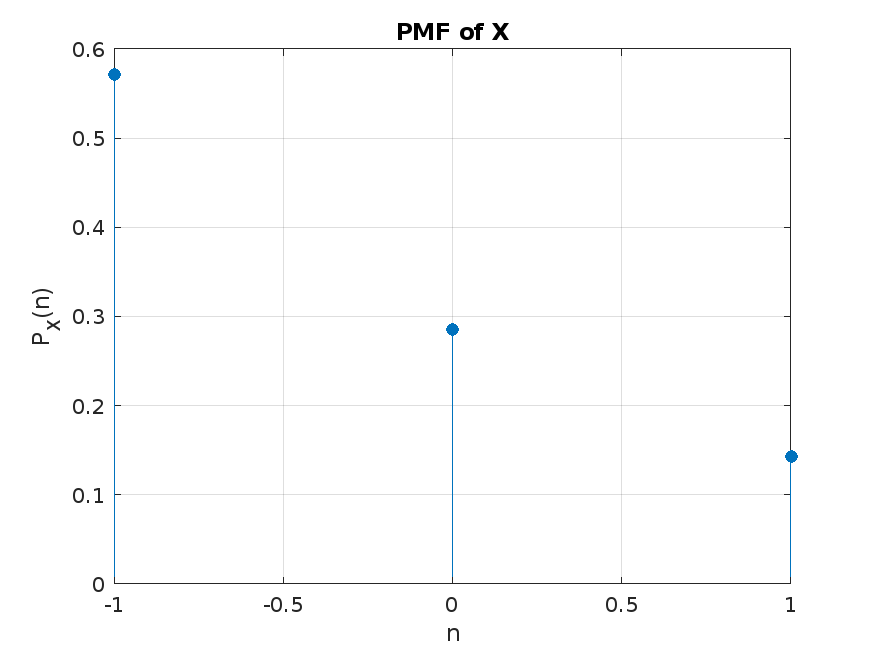
\includegraphics[scale=0.7]{plot_pmf_corrected.png}
\end{center}

\subsubsection*{c) Plot CDF}

\begin{center}
  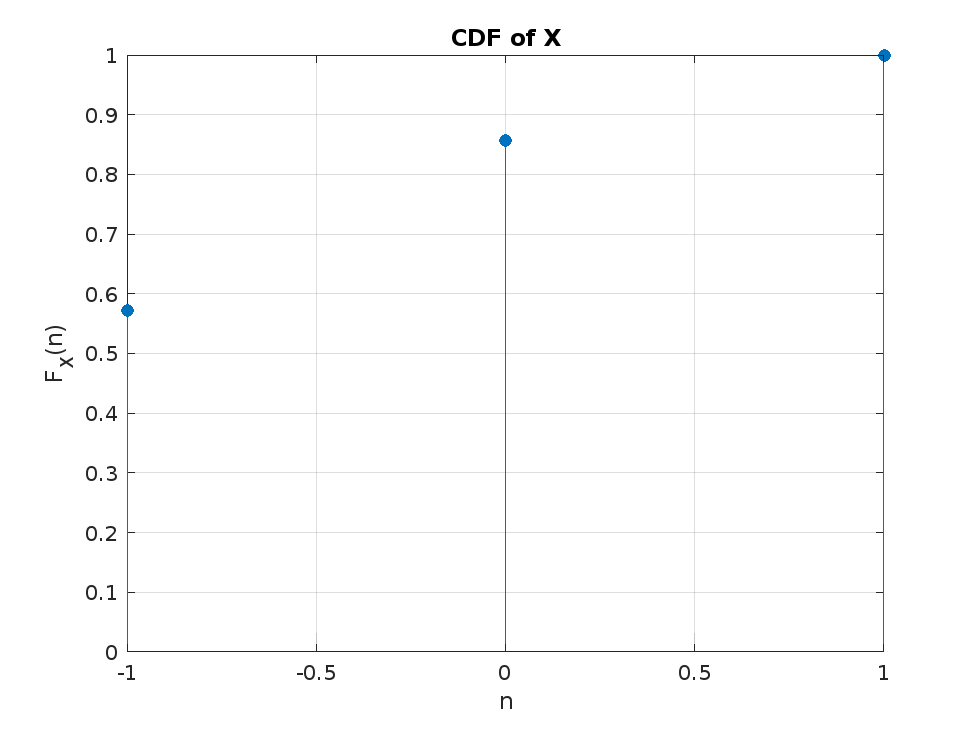
\includegraphics[scale=0.7]{plot_cdf_corrected.png}
\end{center}

\subsubsection*{d) What is \(P(X\leq1)\)?}

\[
P(X\leq 1) = P(X=-1) + P(X=0) + P(X=1) = \frac{2}{7}(2 + 1 + \frac{1}{2}) = \frac{2}{7} \times \frac{7}{2} = 1
\]

\subsubsection*{e) What is \(P(X>0.5)\)?}

\[
P(X > 0.5) = P(X=1) = \frac{2}{7} \times \frac{1}{2} = \frac{1}{7}
\]


\newpage  % Start a new page

\section*{Appendix: MATLAB Code for Generating Plots}

\lstinputlisting[language=Matlab]{code.m}


\end{document}
